\documentclass[12pt,letterpaper,noanswers]{exam}
\usepackage[usenames,dvipsnames,svgnames,table]{xcolor}
\usepackage[margin=0.9in]{geometry}
\renewcommand{\familydefault}{\sfdefault}
\usepackage{multicol}
\pagestyle{head}
\definecolor{c03}{HTML}{FFDDDD}
\header{AM 108 Class 05}{Updated on \today.}{Nondimensionalization}
\runningheadrule
\headrule
\usepackage{graphicx} % more modern
\usepackage{amsmath} 
\usepackage{amssymb} 
\usepackage{hyperref}
\usepackage{tcolorbox}

\begin{document}
 \pdfpageheight 11in 
  \pdfpagewidth 8.5in

\vspace{0.2cm}

\hrule
\vspace{0.2cm}

\begin{itemize}
    \item There is a pre-class assignment for Wednesday (Check Yourself C06).
    \item There is a two question skill check on Wednesday.  The sample questions for it are below.
    \item Before attending OH, post to \#officehours on Slack (or the Office Hours thread on Piazza) to let your classmates and the course staff know what questions / problems you're bringing to OH.
    \item OH this week: 10-11am ET Tuesday, 3-4pm and 7-8:30pm ET Wednesday, 3-4pm (usually 4-5pm) and 8-9:30pm ET Thursday, 3-4pm Friday.  Find the zoom links (and the person staffing the OH) on Canvas.
\end{itemize}

\hrule
\vspace{0.2cm}

\noindent\textbf{Teams}

\begin{multicols}{2}
1. 
\end{multicols}

\noindent \textbf{Teams 1 and 2}: Post screenshots of your work to the course Google Drive today.  Include words, labels, and other short notes that might make those solutions useful to you or your classmates.  Find the link in Canvas (or here: \url{https://drive.google.com/drive/u/0/folders/1GcpwvKHD4tMecpFQ4lNxN_r5Ylj7YHbd})

\vspace{0.2cm}

\hrule
\vspace{0.2cm}

\noindent \textbf{Extra vocabulary / extra facts:}
\begin{tcolorbox}

We will say that a system exhibits \textbf{bistability} if there exist two distinct stable states at the same set of parameter values.  

A \textbf{nondimensional group} is a group of parameters or constants that together are dimensionless but that have the property that any factor of the group has dimension.

A \textbf{Monod function} is a type of switching function (just as $\tanh x$ was an example of a switching function).  The Monod function has the form $f(x) = r\frac{x}{a+x}$.

A \textbf{Hill function} is a type of switching function (compare to $\tanh x$ and to the Monod function).  The Hill function has the form $f(x) = r\frac{x^n}{a^n+x^n}$ where $n$ is the \emph{Hill coefficient}.

\end{tcolorbox}

\eject

\vspace{0.2cm}

\hrule
\vspace{0.2cm}

\noindent\textbf{Addressing your questions}

Nondimensionalization
\begin{enumerate}
\itemsep-0.2em
\item Why do we want to nondimensionalize?
\item What does it mean for something to be non-dimensional?  Why does this process produce something non-dimensional?
\item What does `dimension' in this context have to do with the use of the term `dimension' for the dimension of a space?
\item When nondimensionalizing, why do we isolate the derivative, vs choosing constants that isolate a different term?
\item When we add two quantities, such as $1 + \frac{S}{K}$, why do $1$ and $\frac{S}{K}$ have the same dimension?
\item If we have $\left[\dfrac{S}{K}\right] = 1$, why does that imply $\left[S\right] = \left[K\right]$?
\end{enumerate}

Bistability
\begin{enumerate}
\itemsep-0.2em
\item What do vertical arrows indicate when they are added to a bifurcation diagram?
\item Why do we use discrete stair-steps to dial the parameter, rather than moving smoothly?
\item When we drew an initial example bifurcation diagram for a bistable case (with two saddle-node bifurcations), what did that have to do with the saddle-node example that showed reasoning about $\dot x = f_1(x) - f_2(x)$?
\item Does bistability refer to seeing two different stable states as we shift a parameter, or does it refer to the existence of two different stable states at a particular parameter?
\item For $\frac{dx}{dt} = x\left(r(1-x/k) - \frac{x}{1+x^2}\right)$, how did the graph of $g(x) - f(x)$ connect to the stability diagram?

\end{enumerate}

\vspace{0.2cm}
\hrule
\vspace{0.2cm}


\noindent\textbf{Skill check C06 practice} 
\begin{questions}
\item (retake C03) Let $\dot x = (x-1)(x+2)$

Use \textbf{linear stability analysis} to find the fixed points and to identify their stability. \emph{Show your algebraic work}.  (Work on this Q can replace Skill Check C03).
\item Consider the differential equation \[\frac{dx}{d\tau} = r T_0\left(\frac{1}{h_v}+ x\right)- \frac{r T_0 A}{K} x.\]
Assume that $x$ and $\tau$ are nondimensional variables and that $r, T_0, A, K$ are parameters with dimension.

Identify two nondimensional groups from the equation above.

\bgroup
\def\arraystretch{4}
\begin{tabular}{|p{7cm}|}
\hline
nondimensional groups: \\
\hline\hline
1.\hfill\\
 \hline
2.\hfill \\
 \hline
\end{tabular}
\egroup
\end{questions}

\noindent\textbf{Skill check C06 practice solution} 
\begin{questions}
\item (retake C03) See Skill Check C03 solution on Canvas.
\item $x$ and $\tau$ are nondimensional.  In addition, quantities that are added to each other or are equal to each other must have the same dimensions.

We have $\left[\dfrac{dx}{d\tau}\right] = \left[r T_0\left(\dfrac{1}{h_v}+ x\right)\right] = \left[\dfrac{r T_0 A}{K} x\right]$ (where $\left[ . \right]$ denotes ``the dimensions of'').

We have $\left[x \right] = \left[\tau\right] = 1$.  So $\left[\dfrac{dx}{d\tau}\right] = 1$ (these are all dimensionless).

The dimension of a product is the product of the dimensions, so

$1 = \left[r T_0\right]\left[\left(\dfrac{1}{h_v}+ x\right)\right] = \left[\dfrac{r T_0 A}{K}\right]\left[ x\right]$.

The dimension of a sum is the dimension of either component of the sum, so

$1 = \left[r T_0\right]\left[x\right] = \left[\dfrac{r T_0 A}{K}\right]\left[ x\right]$.

Using $\left[x \right] = 1$, this is $1 = \left[r T_0\right] = \left[\dfrac{r T_0 A}{K}\right]$.

$rT_0$ is a dimensionless group.  $1 = \left[\dfrac{r T_0 A}{K}\right] = \left[rT_0\right]\left[\dfrac{A}{K}\right]$.  $\dfrac{A}{K}$ is another dimensionless group.  $h_v$ is a dimensionless parameter (but is not a group).


\end{questions}


\vspace{0.2cm}

\hrule
\vspace{0.2cm}
\noindent\textbf{Nondimensionalization}
\begin{questions}
\item Let $\dot{N} = r N (1-N/K) -H$.  This is a logistic population model where there is a constant harvesting rate reducing population growth.

\begin{parts}
\item For each of the variables and each of the parameters, identify its associated dimension.  \emph{Write this out in expressions of the form $[a] = L$.}
\item Create dimensional constants, $N_0$ and $T_0$, and use them to create nondimensional
variables $x = N/N_0$ and $\tau = t/T_0$.  Substitute $x$ and $\tau$ into the equation and simplify.

\item List all nondimensional groups that arise.  Consider a combination a \emph{nondimensional group} if the combination is nondimensional but every piece would be dimensional if it were broken apart in any way.

\textbf{Teams 3 and 4, post your non-dim groups and a brief description of your process to the \#classactivities thread on Slack (your work on parts abc above)}.
% \item Check your work with a nearby team.
\item Make choices for values of the constants $T_0$ and $N_0$ that eliminate two of the nondimensional groups.
\item Define a new nondimensional parameter (use a Greek letter such as $\alpha, \beta, \gamma, \mu$), and rewrite your equation as a nondimensional one.
\item How many parameters are there in the nondimensional system?  
How does this compare to the number in the dimensional version?
 Notice that each dimensional constant we introduce enables us to remove a parameter, so that the nondimensional equation has fewer parameters than the dimensional one.  \emph{This result on the reduction in the number of parameters from nondimensionalization is called the Buckingham Pi theorem.  It is called the ``pi'' theorem because he used the symbols $\Pi_1$, $\Pi_2$, etc to represent the nondimensional groups.}
 
 \textbf{Teams 5 and 6, post info about the nondimensionalization you chose to the \#classactivities thread on Slack (your work on parts def above)}.
\end{parts}
\item Let $\dot{N} = r N (1-N/K) - H N/(A+N)$.  This is a slightly different harvesting case.  
\begin{parts}
\item This harvesting term, $HN/(A+N)$, is in the form of a special function called a \textbf{Monod function}.  Plot an approximation of the Monod function by hand \textbf{without} using any plotting tools.  
\item What do you think of this function as a description of a harvesting process?
 
 %{2019: \color{blue} Many groups got to this point or were working on this plot.}
\item Identify the dimension of each of the variables and parameters.  Once you nondimensionalize
how many parameters do you expect to remain?
\item Nondimensionalize this equation.  
\begin{itemize}
    \item As part of this process, identify the dimensionless groups and check your work with another team.
    \item There are multiple good choices for $N_0$.  What are some
reasons to choose one or the other?
\end{itemize}
\item Now that it's nondimensional, take another look at the expression for your harvesting function.  Plot it using appropriate axis ticks.  How did your axis tick labels change?
\end{parts}

\emph{hints for plotting the monod function:}

\begin{itemize}
    \item How does the function behave as $N\rightarrow 0$?  
    \item How does it behave as $N \rightarrow \infty$?
    \item Use a unit increment of $A$ on the horizontal axis and an increment of $H$ on the vertical axis.  Mark the point corresponding to an input of $N = A$.
    \item Find the slope of the function at $N = 0$.  \emph{What do you expect it to be?}  For your reference: $\displaystyle\frac{d}{dN}(H N/(A+N)) = \frac{H}{A+N}-\frac{HN}{(A+N)^2}.$
    \item Draw a curve that connects up the features you have identified.
\end{itemize}
\end{questions}
\end{document}





% \vfill
% \begin{questions} 
% \item Let $\dot{N} = RN(1-N/K) - BN^2/(A^2+N^2)$.  This model is describing spruce budworms
% growing on spruce trees and facing predation by birds.  On the timescale of the budworm growth,
% the tree and bird populations are thought of as constant.
% \begin{parts}
% \item This is a lot of practice with very similar equations, but here goes: how is the predation
% term in this model different from the harvesting term in the model above?
% \item Nondimensionalize, choosing $N_0$ and $T_0$ so that the nondimensional equation is
% \[\frac{dx}{d\tau} = r x \left(1-\frac{x}{k}\right) - \frac{x^2}{1-x^2}.\]
% \end{parts}
%{2018: \color{blue} Many groups got to this point.}

\item  Choose a nondimensional model from the ones you've constructed and begin a bifurcation analysis.
%Back to bifurcation: 
%\item (3.7.3) Consider the system $\dot{x} = x(1-x) - h$, which is a dimensionless model of 
%a fish population under harvesting.  
%\begin{parts}
%\item Show that a bifurcation occurs at some value of the parameter, $h_c$, and classify the bifurcation.
%\item What happens at long times to the fish population for $h<h_c$, and for $h>h_c$?
%\end{parts}


% \item Consider the spruce budworm model $\dot{x} = rx(1-x/k) - x^2/(1-x^2)$.
% \begin{parts}
% \item 
% \begin{figure}[h]
% \begin{center}
% 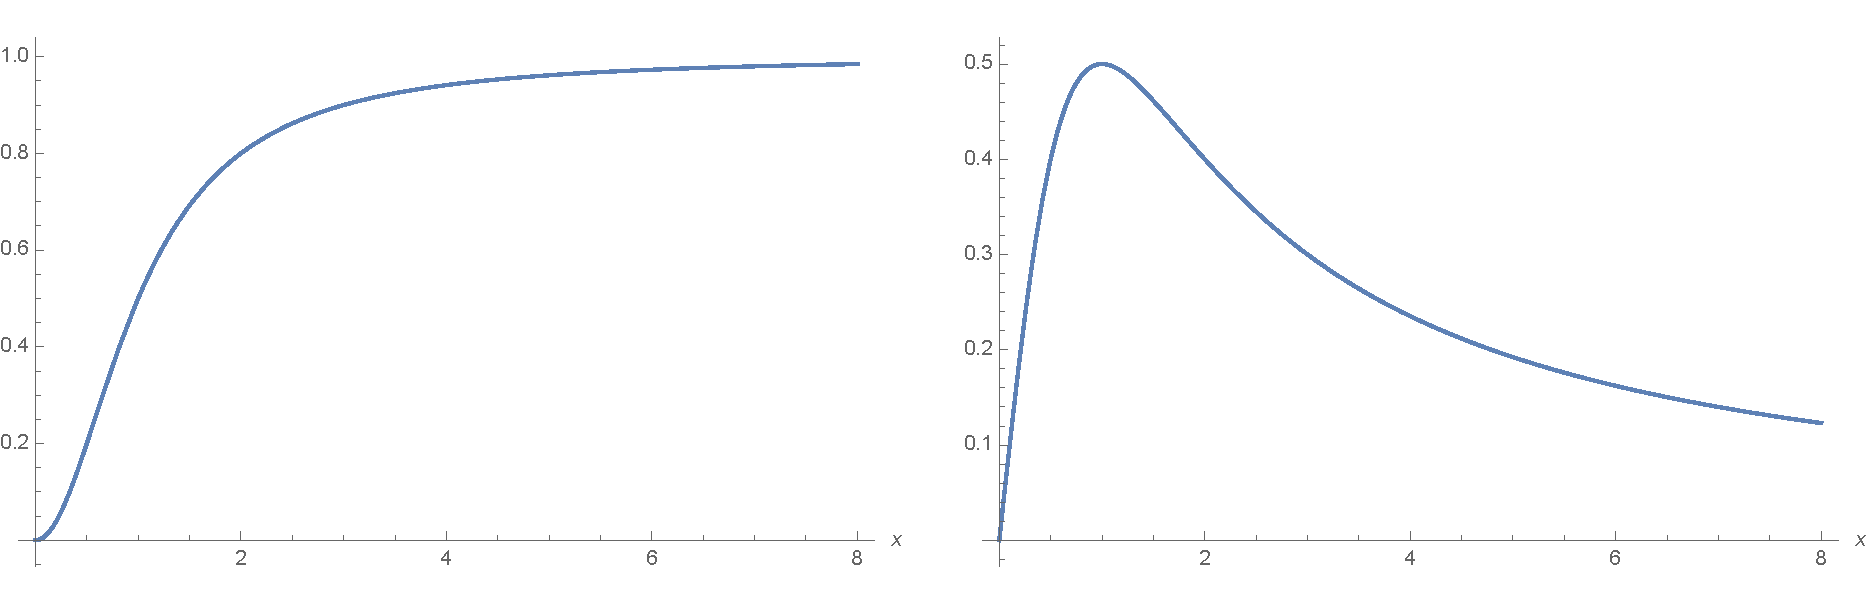
\includegraphics[scale=0.4]{img/HillFunction.pdf}
% \caption{On the left is a plot of $x^2/(1-x^2)$ while on the right is a plot of $x/(1-x^2)$.}
% \end{center}
% \end{figure}
% Use the plots to argue that the system can have one, two, or three fixed points, depending on
% values of $r$ and $k$.
% \item Identify what kinds of bifurcations occur in this system.  It is fine to reason this out based on the plot.
% \item Sketch lines in the $kr$ plane to show the parameter sets where 
% there is an outbreak of budworms, 
% the sets where the budworms remain at a low (termed {\it{refuge}}) level, 
% and those where there is bistability between the two cases.  This sketch in parameter space is a \emph{stability diagram}.
% \end{parts}



%\item (3.7.4) Consider the system $\dot{x} = x(1-x) - hx/(a+x)$.  This is a dimensionless model of a fish
%population under harvesting and is more sophisticated than the model above.  
%\begin{parts}
%\item Analyze the dynamics near $x=0$ and show that a bifurcation occurs when $h = a$.
%What kind of bifurcation is it?
%\item Show that another bifurcation occurs when $h = \frac{1}{4}(a+1)^2$ for $a<a_c$ where
%$a_c$ is to be determined.  Classify this bifurcation.
%\item Plot the stability diagram of the system in the $ah$-plane.  Identify whether there are any
%regions where we expect hysteresis to occur.
%\end{parts}
\end{questions}


\end{document}